% Author: Tilman Rassy <rassy@math.tu-berlin.de>
% $id$

% $Id: praes.tex,v 1.2 2007/10/14 01:03:00 rassy Exp $

\documentclass{article}

\usepackage{ngerman}
\usepackage{amssymb,amsbsy}
\usepackage[pdftex,pdfpagemode=None,bookmarks=false,colorlinks=true,linkcolor=blue]{hyperref}
\usepackage{epsfig}
\usepackage[display]{texpower}
\usepackage{color}

% Author: Tilman Rassy <rassy@math.tu-berlin.de>
% $Id: macros.tex,v 1.5 2006/10/05 15:58:42 rassy Exp $

% XML code:
\newcommand{\element}[1]{\code[xml-element]{#1}}
\newcommand{\attrib}[1]{\code[xml-attrib]{#1}}

% Database code:
\newcommand{\dbtable}[1]{\code[db-table]{#1}}
\newcommand{\dbcol}[1]{\code[db-column]{#1}}
\newcommand{\sql}[1]{\code[sql]{#1}}

% TeX code:
\newcommand{\texcmd}[1]{\code[tex-cmd]{\backslash#1}}
\newcommand{\texenv}[1]{\code[tex-env]{#1}}

% General
\newcommand{\val}[1]{\code[value]{#1}}
\newcommand{\prm}[1]{\code[param]{#1}}

% Other:
\newcommand{\notimpl}[1]{\emph[not-impl]{#1}}
\newcommand{\new}[1]{\emph[new]{#1}}
\newcommand{\deprecated}[1]{\emph[deprecated]{#1}}
\newcommand{\wvar}[1]{\var[weak]{#1}}


\hoffset0cm
\voffset0cm
\topmargin0cm
\headheight0cm
\headsep0cm
\topskip0cm
\marginparwidth0cm
\marginparsep0cm

\paperheight16cm
\paperwidth20cm
\textheight14cm
\textwidth16cm

\oddsidemargin0mm
\evensidemargin0mm

\nonfrenchspacing
\parindent0em
\parskip0.2\baselineskip

\pagestyle{empty}

\sloppy

\begin{document}

\sffamily

\pagebreak

\begin{center}

\textbf{\color{headlinecolor}\titlesize 
Web-2-Technologien fuer eine multimediale Lernplatform}

\vspace{1.0cm}

\normalsize
Tilman Rassy

\vspace{1.0cm}

Technische Universit"at Berlin \\
Fakult"at II -- Mathematik und Naturwissenschaften \\
Institut f"ur Mathematik

\end{center}

\pagebreak

\mysection{Was ist MUMIE?}

\begin{mylist}

\pitem E-Learning-Plattform f"ur Mathematik

\pitem Funktionalit"aten:
\begin{mylist}[\mylabelitemii]
  \pitem Darstellung mathematischer Inhalte: Wissensbausteine,
         erg"anzt durch Bemerkungen, Beispiele, Visualisierungen (Multimedia)
  \pitem Aufgaben: verschiedene Typen; individualisiert; automatisch
         korrigiert und bewertet
  \pitem Strukturiert in Kursen
  \pitem Autorentools
\end{mylist}

\pitem Open-Source-Projekt
\begin{mylist}[\mylabelitemii]
  \pitem TU Berlin, Institut f"ur Mathematik
\end{mylist}

\end{mylist}

\pagebreak

\mysection{Was ist MUMIE?}

\begin{center}
\hspace*{-0.5cm} 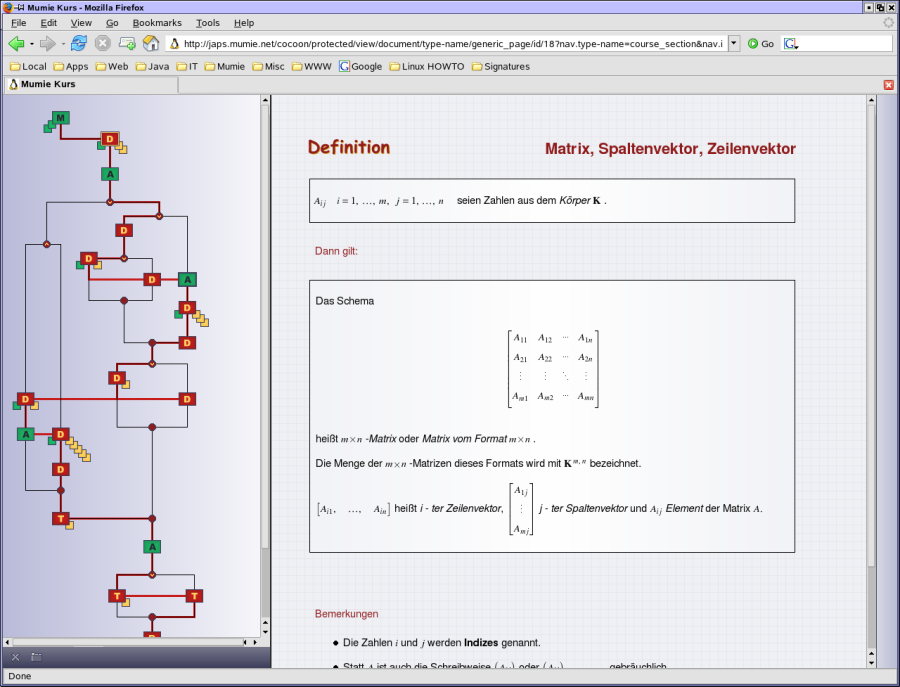
\includegraphics[width=16cm]{mumie_screenshot_01}
\end{center}

\pagebreak

\mysection{Was ist MUMIE?}

\begin{center}
\hspace*{-0.5cm} 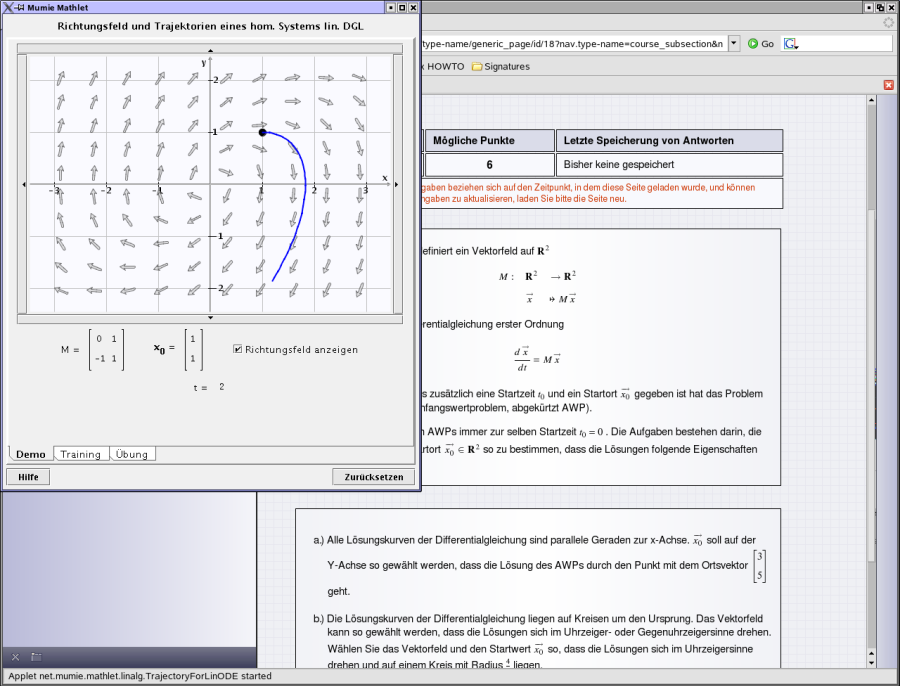
\includegraphics[width=16cm]{mumie_screenshot_02}
\end{center}

\pagebreak

\mysection{MUMIE -- Technisches}

\begin{mylist}

\pitem Technologie:
\begin{mylist}[\mylabelitemii]
  \pitem Java-Servlet-Technologie
  \pitem XML-Technologie
  \pitem Dynamische Seitenerzeugung
\end{mylist}

\pitem Architektur:
\begin{mylist}[\mylabelitemii]
  \pitem Apache (Webserver)
  \pitem Tomcat (Servlet-Container)
  \pitem Cocoon + MUMIE-eigene Komponenten (Servlet)
  \pitem PostgreSQL (Datenbank) 
\end{mylist}

\end{mylist}

\pagebreak

\mysection{MUMIE -- Technisches}

\vspace{2cm}

\hspace*{-1.5cm}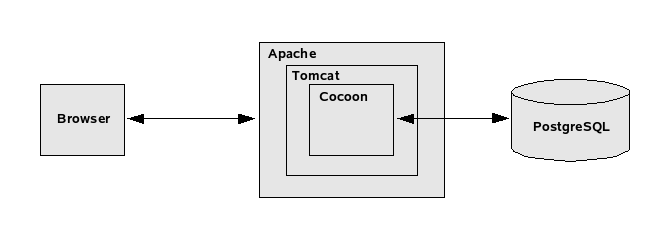
\includegraphics{arch_mumie}

\pagebreak

\mysection{MUMIE -- Geschichte}

\begin{mylist}

\pitem 2001 - 2004: Kooperationsprojekt der TU Berlin, Uni Potsdam, RWTH
        Aachen und TU M"unchen, gef"ordert durch das BMWF
\pitem Seit 2004: Fortgef"uhrt an der TU Berlin in loser Zusammenarbeit mit
       der RWTH Aachen und TU M"unchen
\pitem Ab Sommersemester 2005 Testeins"atze an der TU Berlin; ab Wintersemester
       2006/2007 regul"arer Einsatz (Lineare Algebra f"ur Ingenieure, 2000 H"orer)
\pitem Einsatz an der TU M"unchen
\pitem Ab Herbstsemester 2007 Einsatz an der ETH Z"urich

\end{mylist}

\pagebreak

\mysection{Was ist Web 2.0?}

\begin{mylist}

\pitem \glqq 2.0\grqq\ ist keine Software-Versionsnummer

\pitem Vager Begriff; keine pr"azise Definition

% \pitem Popul"ar gemacht von Tim O'Reilly

\pitem Bisher: Feste, wenig interaktive Webseiten;\pause Web 2.0: stark
interaktive Webseiten, Inhalt von Benutzern mitgestaltet

\pitem Neue Technologie: Ajax \pause (Asynchronous JavaScript and XML)

\pitem Erlaubt es, Webseiten mit Eigenschaften von Desktop-GUIs auszustatten

\pitem Neuere Entwicklungen: Java FX, Adobe AIR, Silverlight

\end{mylist}

\pagebreak

\mysection{MUMIE und Web 2.0}

\begin{mylist}
\pitem Bisher keine Web-2.0-Technologie in der MUMIE
\pitem Projektaufgaben:
\begin{mylist}[\mylabelitemii]
  \pitem Erarbeitung von Vorschl"agen f"ur den sinnvollen Einsatz von Web 2.0
         in der MUMIE
  \pitem Konzeption und Implementation von einem oder mehreren Beispielen
\end{mylist}
\end{mylist}

\end{document}
